\section{System design and implementation}
\label{sec:implementation}

\begin{figure}
  \centering
  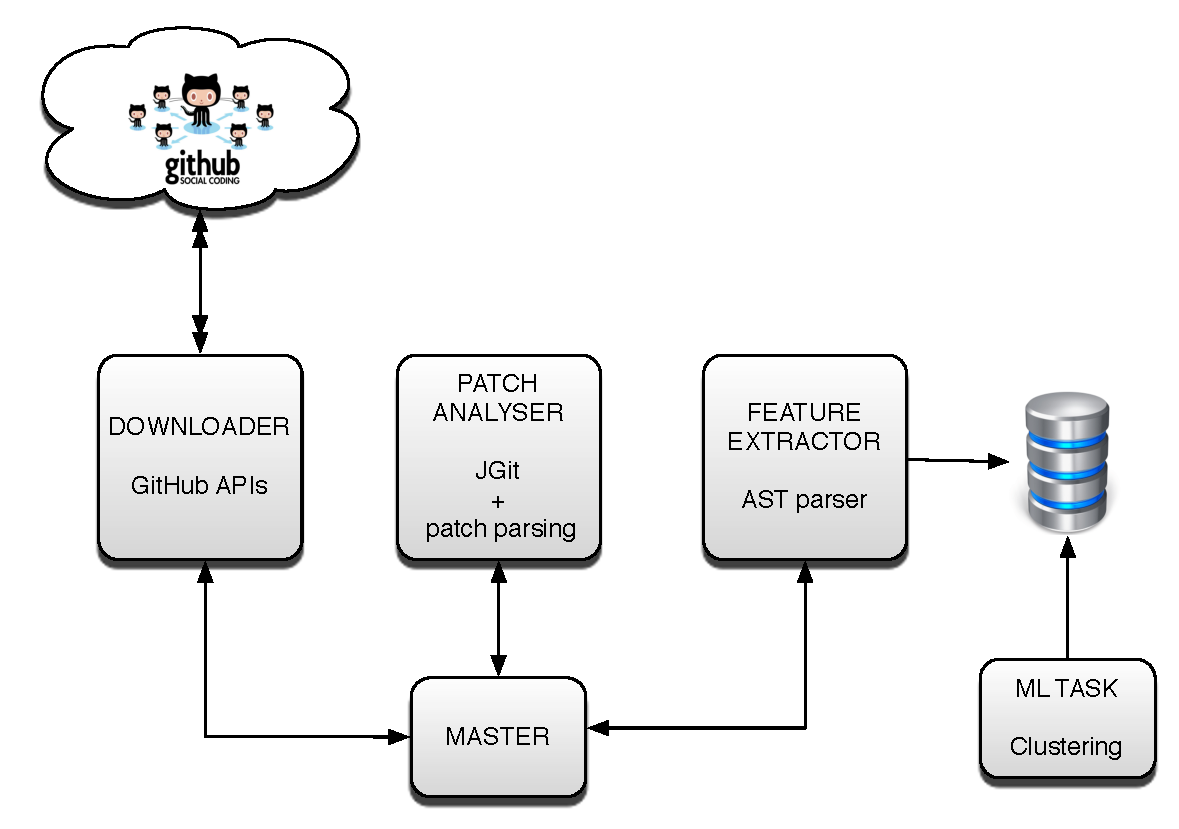
\includegraphics[width=0.5\textwidth]{pictures/overallArch.pdf}
  \caption{Overview of the proposed approach}
  \label{fig:overall}
\end{figure}


The system was thought taking into account two main features: scalability and high patch-analysed ratio. In order to achieve these two goals the system was designed as what we define: a replicable and single stage scalable pipeline. The main idea, as shown in Figure \ref{fig:overall}, is to have a pipeline of stages that are in charge to download repositories and issues related to them, then to extract patches from those and then mix the just retrieved data in order to extract features for the machine leaning task. In order to improve the scalability, the development and future extension every stage was developed independently from the others. In this direction we adopted reactive programming paradigm using the Akka framework, defining each stage as an actor. Those actors are of three kinds, one for each stage of the pipeline: the downloader, the patch-analyser and the feature-extractor. Actually there is a fourth actor -the master- in charge to manage the communication flow between the others and to instantiate new actors if needed. The pipeline is meant to be replicable in the sense that instantiating more than one stage at time it's possible to have several pipelines working in parallel. The mean of single stage scalable lies in the fact that it is also possible to set the number of replicas of a single stage independently by the other two. This means that in case a stage is slower than the others, just replicate its functionalities with one more actor of the same kind and in this way the bottleneck will be less strict. All of these parameters can be fixed inside a configuration class, which contains parameters for a full customization of the system. The output of the pipeline is a dataset representing a set of features describing the changes made in order to fix an issue in the repository. These data are then used to feed the machine learning task, that tries to find common pattern between changes and try to cluster them together. In this section we are going to go deep into each pipeline's stage and its duties. 
\subsection{Downloader}
This stage of the pipeline is in charge to directly manage the GitHub APIs. These are REST APIs based on the weel known JSON format. In detail the system exploits REST call with OAuth authorization in order to increase the number of request per hour allowed (5000). The first request the downloader makes is for retrieving a list of issues that were closed. Once those are retrieved via parsing the JSON response they are filtered, all meaningless ones are discarded, where meaningless means those issues related to repositories not public or where the coommit that closed those issues is missing. In order to retrieve the information necessary to the filter step different API calls are made and the responses are mixed together in order to extract the necessary parameters for the filter. Once the repo is marked as good the downloader downloads it and send information to local repository path, relative issue and closing commit to the patch analyser stage. 
\subsection{Patch Analyser}
This stage of the pipeline is in charge of extracting the modifications introduced by a commit, given a commit hash from the previous stage. We take advantage of the JGit library to extract the location of the modifications performed by the commit in the source code.
\subsection{Feature Extractor}
This stage of the pipeline receives information about diffs in a patch file and extracts features from the involved source files. The goal is to obtain a numerical dataset where each sample represents a single diff in a patch file. First, the files before and after the change are parsed to generate their AST. Then, the AST is used to extract features from the portion of code that has changed. We define a feature as the number of occurrences of some semantic attribute in the code (e.g., a for loop, a certain operation, a lambda expression, and so on). A sample is then the vector of features in the code before and after the change. Thus, we obtain a (very sparse) numerical dataset onto which we can apply clustering techniques. 
\subsection{Machine Learning} 
We apply clustering on the numerical dataset generated by our system. We decided to consider only hierarchical clustering since it provides the most general results (we get a cluster dendogram that we can cut in the desired number of clusters). We adopt the cosine similarity measure since it is the most suitable for our kind of dataset (high-dimensional and sparse feature vectors). We implement our clustering script in R, so that it can be easily integrated with Spark in case we need to scale to larger datasets.